\chapter{Naivni Bayes}
\label{ch:naivni-bayes}

\begin{wrapfigure}{o}{0.6\textwidth}
    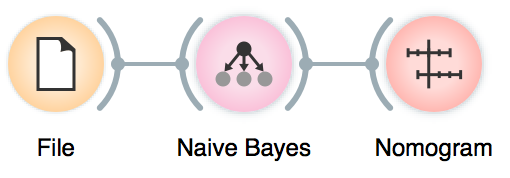
\includegraphics[scale=0.7]{workflow.png}
    \caption{$\;$}
\end{wrapfigure}

Poglejmo si še nekaj drugih klasifikacijskih metod, npr. naivnega Bayesa. Tokrat bomo poskušali napovedati, kateri od potnikov Titanika, ki je potonil sredi Atlantskega oceana leta 1912, so preživeli. \textit{titanic.tab} opisuje 2201 potnika, njegovo vozovnico (prvi, drugi, tretji razred, osebje), starost in spol.

Naložimo podatke in jih peljimo v gradnika \widget{Naive Bayes} in \widget{Nomogram}.

\marginnote{Naivni Bayes je metoda, ki predpostavlja (glede na razred) med seboj neodvisne spremenljivke. Če bi bile spremenljivke med samo neodvisne - kar so v praksi redko - bi bil naivni Bayes idealni klasifikator.}V Nomogramu vidimo lestvico ‘Points’ na vrhu in lestvice za vsako spremenljivko posebej (skupaj tri). Spodaj je dvojna lestvica verjetnosti. Pozorni bodite na ‘Target class’ v zgornjem levem kotu. Če nastavimo ciljno vrednost na ‘yes’, potem bo nomogram prikazal verjetnost, da je potnik preživel.

Iz nomograma je razvidno, da je za naivnega Bayesa najpomembnejša spremenljivka spol. Če premaknemo modro točko na ‘female’, vidimo, da se verjetnost za preživetje poveča na 73 \%. Če je ta ženska potovala v prvem razredu, se njena možnost preživetja poveča na 90 \%. \marginnote{Nomogram sešteje prispevke vsake spremenljivke k ciljni vrednosti (preživetje) in potem to pretvori v verjetnost.}Za napovedi potrebujemo vsoto vseh prispevkov k ciljni vrednosti (preživetje) in nato to pretvorimo v verjetnost. Pretvorba je prikazana na spodnji lestvici.

\begin{figure*}[h]
    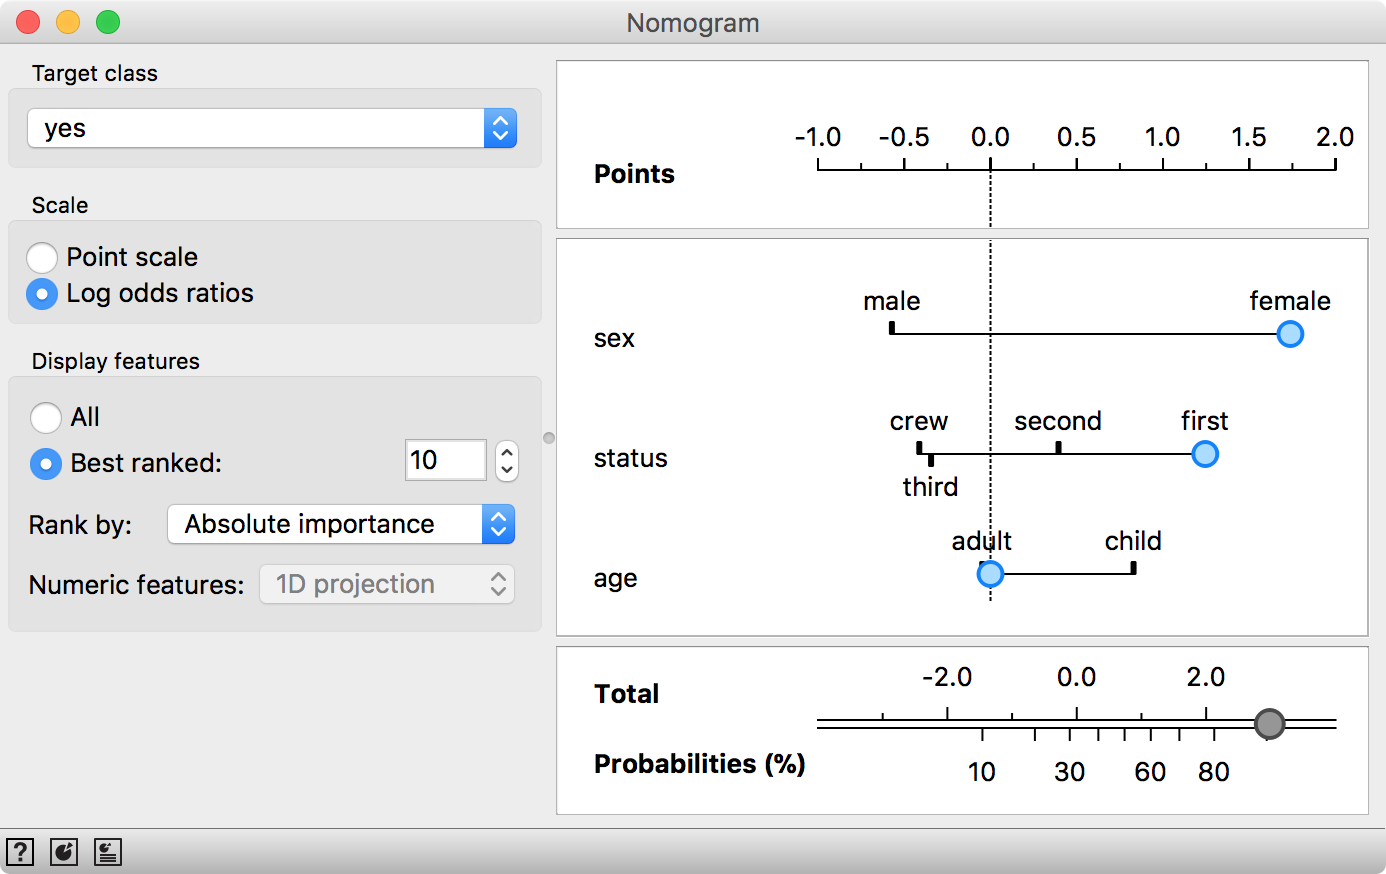
\includegraphics[width=0.8\linewidth]{nomogram.png}
    \caption{$\;$}
\end{figure*}

\newpage

Vrnimo se k podatkom \textit{brown-selected.tab}. Da bi Naive Bayes delal na teh podatkih, moramo številske spremenljivke pretvoriti v kategorične.\marginnote{Ali še vedno razumemo model?}

\begin{figure*}[h]
    \centering
    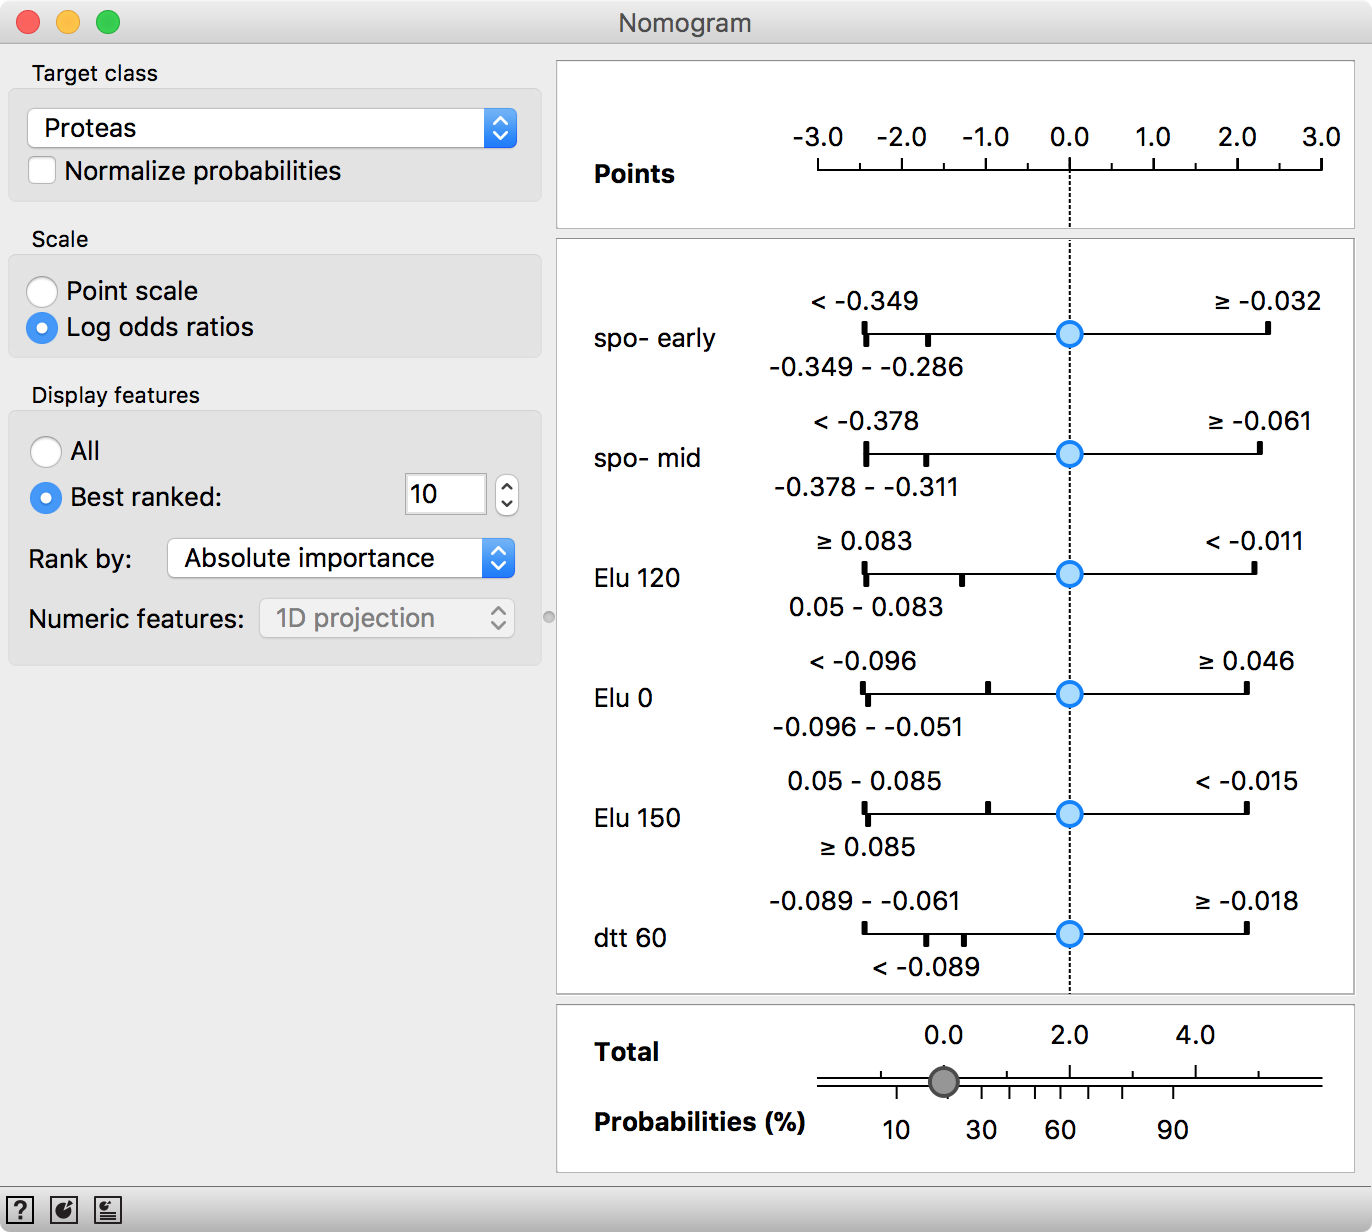
\includegraphics[width=0.8\linewidth]{nomogram2.png}
    \caption{$\;$}
\end{figure*}

Ko pretvorimo številke v kategorije, izgubimo določeno mero preciznosti, ki lahko vpliva na točnost modela. In ker so številke sedaj predstavljene kot grobi intervali, iz nomograma težko razložimo model.

Poglejmo si raje metodo, ki odlično dela s številskimi vrednostmi, hkrati pa jo lahko enako lepo prikažemo.